% !TEX program = pdflatex
% !TEX options = --shell-escape "%DOC%"

% Before compiling :
% * Ensure convert is in path (ImageMagick)
% * Ensure gs is in path (Ghostscript)
% * Ensure that you have gs≥9.24 and ImageMagick 6+
%     * convert --version
%     * gs --version
% * Check for vulnerability policies in ImageMagick : https://stackoverflow.com/a/59193253/7767136
% * Compile with --shell-escape


% Converting with standalone
% Same as convert -density 600 document.pdf -quality 90 figure.png
% Default param for quality is 90
\documentclass[tikz, border=7pt, convert={density=600, png}]{standalone}


% Block diagrams & Flowcharts
% ========================================
\usepackage{tikz}
\usetikzlibrary{shapes,arrows}
\usetikzlibrary{calc,positioning}
\tikzstyle{arrow} = [thick,->,>=latex']

\tikzset{
    block/.style = {draw, fill=white, rectangle, minimum height=2em, minimum width=2em},
}


% % White page color for pictures
\usepackage{xcolor}
\pagecolor[HTML]{FFFFFF}



\begin{document}
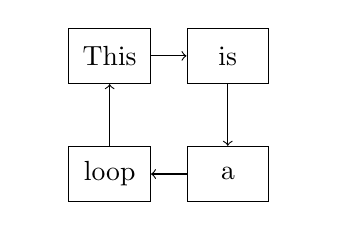
\begin{tikzpicture}[auto, node distance=1.5cm, text width=0.8cm, align=center]
    \node [block] (this) {This};
    \node [block, right of=this] (is) {is};
    \node [block, below of=is] (a) {a};
    \node [block, left of=a] (loop) {loop};

    \draw [->] (this) -- node {} (is);
    \draw [->] (is) -- node {} (a);
    \draw [->] (a) -- node {} (loop);
    \draw [->] (loop) -- node {} (this);
\end{tikzpicture}

\end{document}



